\documentclass[conference]{IEEEtran}
\usepackage{cite}
\usepackage{amsmath,amssymb,amsfonts}
\usepackage{algorithmic}
\usepackage{graphicx}
\usepackage{textcomp}
\usepackage{xcolor}
\usepackage{booktabs}
\usepackage{multirow}
\usepackage{url}

\def\BibTeX{{\rm B\kern-.05em{\sc i\kern-.025em b}\kern-.08em
    T\kern-.1667em\lower.7ex\hbox{E}\kern-.125emX}}

\begin{document}

\title{FGEAD: A Feature-Level Graph-Based Framework for Explainable Anomaly Detection in Multivariate Time Series}

\author{
\IEEEauthorblockN{SAIKRISHANSIVARAM NANDIGAM}
\IEEEauthorblockA{Enrollment No.: 2303031241180}
\and
\IEEEauthorblockN{Chinthala Yuva Kishore}
\IEEEauthorblockA{Enrollment No.: 2303031240325}
\and
\IEEEauthorblockN{MAGANTI SALMAN RAJU}
\IEEEauthorblockA{Enrollment No.: 2303031240605}
}
\maketitle

\begin{abstract}
Detecting anomalies in high-dimensional multivariate server telemetry is critical for maintaining infrastructure reliability. However, deep learning anomaly detection models often function as opaque black boxes, failing to explain why an observation was flagged or which metric relationships altered. In this paper, we present \textbf{FGEAD} (Feature-level Graph-based Explainable Anomaly Detection), an end-to-end semi-supervised forecasting framework equipped with an integrated post-hoc explainability engine. FGEAD models evolving inter-metric topological dependencies using a self-attention graph learner with Top-$K$ sparsification ($K=5$), combined with Graph Convolutional Networks (GCN) and a 2-layer LSTM for spatio-temporal representations. Anomaly detection is performed via next-timestep forecasting error weighted by learnable feature importance parameters. To address the explainability gap, FGEAD implements a structured 5-question XAI framework: (1) metric deviation ranking via Z-scores, (2) scale-aware directional labeling ($\uparrow$ spike / $\downarrow$ drop), (3) Graph Relationship Auditing contrasting learned attention-derived dependency weights against observed Pearson correlations to isolate decoupling and sign-reversal events, (4) temporal range localization, and (5) composite confidence scoring. Evaluated on the benchmark Server Machine Dataset (SMD Machine 1-1, 38 metrics, 28,479 test timesteps), FGEAD achieves a window-level ROC-AUC of 0.9709, PR-AUC of 0.7981, Recall of 0.9039, and F1-score of 0.6916 (Point-level ROC-AUC 0.9708, Recall 0.9714). The high recall reflects a deliberate operational threshold calibration (99.5th percentile) favoring anomaly sensitivity. FGEAD is deployed via a FastAPI REST backend and a Streamlit observability dashboard prototype.
\end{abstract}

\begin{IEEEkeywords}
Explainable AI (XAI), Anomaly Detection, Graph Neural Networks, Multivariate Time Series, Server Telemetry, Graph Relationship Auditing, Feature Attribution.
\end{IEEEkeywords}

\section{Introduction}
Modern cloud infrastructures and enterprise server clusters generate continuous streams of multivariate telemetry data, spanning CPU utilization, memory pressure, disk I/O, network throughput, and kernel performance metrics \cite{wang2025survey}. Rapid identification of operational anomalies is vital to mitigate system outages, service degradation, and hardware failures \cite{su2019omnianomaly}. 

While deep learning architectures—such as Autoencoders, Recurrent Neural Networks (RNNs), Transformers, and Graph Neural Networks (GNNs)—have demonstrated strong detection capabilities \cite{audibert2020usad, xu2022anomaly, deng2021graph}, their operational utility is often hindered by the ``black-box'' problem \cite{barredo2020explainable, rudin2019stop}. When an automated monitoring tool triggers an alert on a 38-metric server telemetry stream, site reliability engineers (SREs) and operations teams need to address critical diagnostic questions: \textit{Which specific metrics deviated? What were their expected values? Have dependency patterns between components changed? How confident is the alert?}

Applying generic Explainable AI (XAI) feature-attribution tools such as LIME \cite{ribeiro2016why} and SHAP \cite{lundberg2017unified} to multivariate temporal telemetry presents notable challenges. In time-series server metrics, features are frequently strongly interdependent, temporal context is paramount, and local perturbation schemes can produce unrealistic metric states. Furthermore, applying iterative feature attribution over continuous sliding windows carries substantial computational overhead \cite{ying2019gnnexplainer}, while raw importance vectors do not automatically provide relationship-level context or operational alerts \cite{tripathy2022explaining}. Importantly, Jain and Wallace \cite{jain2019attention} demonstrated that internal neural attention weights alone do not reliably constitute complete explanations. \textbf{FGEAD does not use SHAP or LIME}; rather, it implements a specialized, scale-aware post-hoc auditing pipeline tailored for graph-augmented temporal forecasting.

FGEAD unifies high-sensitivity anomaly detection with structured post-hoc diagnostics. FGEAD learns dynamic spatial dependencies between metrics using multi-head self-attention with Top-$K$ sparsification ($K=5$) and L1 regularization, coupled with Graph Convolution (GCN) and Long Short-Term Memory (LSTM) networks to capture temporal sequence dynamics. Anomaly scoring is formulated as a semi-supervised next-step forecasting error weighted by learnable metric importance parameters.

FGEAD integrates a post-hoc explainability engine based on a structured 5-Question Framework. Rather than relying solely on raw feature weights or generic perturbation models, FGEAD performs:
\begin{enumerate}
    \item \textbf{Feature Deviation Analysis:} Standardizing forecast deviations into Z-scores on the original data scale to identify top contributing metrics.
    \item \textbf{Graph Relationship Auditing:} Comparing the model's learned attention-derived dependency matrix against the empirical Pearson correlation matrix of the anomalous window to detect structural dependency breaks (decoupling, sign reversal).
    \item \textbf{Temporal Localization \& Confidence Calibration:} Isolating contiguous anomaly boundaries and computing a multi-factor composite alert confidence score.
\end{enumerate}

The principal contributions of this work are summarized as follows:
\begin{itemize}
    \item We present an integrated spatio-temporal architecture combining dynamic self-attention graph learning, GCN, and LSTM for semi-supervised multivariate time-series anomaly forecasting.
    \item We introduce a Graph Relationship Auditing mechanism that identifies discrepancies between learned dependency representations and observed empirical correlations in anomalous windows.
    \item We define a structured 5-question XAI engine that translates model predictions into actionable alert reports featuring Z-score rankings, directional indicators ($\uparrow/\downarrow$), relationship change types, and composite alert confidence levels.
    \item We conduct empirical evaluations on the benchmark Server Machine Dataset (SMD Machine 1-1) and a 20-feature synthetic telemetry dataset, demonstrating a window-level ROC-AUC of 0.9709 and Point-level Recall of 0.9714.
    \item We provide a prototype deployment implementation featuring a FastAPI REST backend and a Streamlit observability dashboard.
\end{itemize}

\section{Related Work}

\subsection{Explainable Artificial Intelligence (XAI)}
The field of XAI has evolved rapidly to address model interpretability in high-stakes domain deployments \cite{barredo2020explainable}. Model-agnostic post-hoc explanation methods, such as LIME \cite{ribeiro2016why} and SHAP \cite{lundberg2017unified}, rely on local surrogate approximations or game-theoretic Shapley values. Influence functions \cite{koh2017understanding} trace model predictions back to influential training instances. However, Rudin \cite{rudin2019stop} argued that post-hoc explanations on black-box models can be misleading and advocate for domain-aware interpretable design. In multivariate time series, standard feature attribution tools suffer because metrics are strongly correlated and temporal context must be preserved.

\subsection{Machine Learning for Anomaly Detection}
Unsupervised and semi-supervised deep learning models dominate time-series anomaly detection. OmniAnomaly \cite{su2019omnianomaly} introduced stochastic recurrent neural networks with planar normalizing flows alongside the benchmark Server Machine Dataset (SMD). USAD \cite{audibert2020usad} employed adversarial autoencoders to amplify reconstruction errors. MSCRED \cite{zhang2019deep} constructed multi-scale signature matrices processed via ConvLSTM networks. Anomaly Transformer \cite{xu2022anomaly} introduced association discrepancy between prior-associations and series-associations in self-attention. While effective at detection, these methods do not explicitly map feature-to-feature graph topologies alongside structured diagnostic reports.

\subsection{Explainable Anomaly Detection}
Recent research explicitly addresses root-cause localization in anomaly detection. MTAD-GAT \cite{zhao2020multivariate} used dual graph attention networks (feature and temporal) to model metric dependencies. GDN \cite{deng2021graph} inferred directed feature dependency graphs using structure learning to spot relationship deviations. InterFusion \cite{li2021multivariate} utilized hierarchical variational autoencoders with MCMC-based metric localization. GANF \cite{dai2022graph} integrated Bayesian graph discovery with normalizing flows. Exathlon \cite{jacob2021exathlon} established a benchmark framework for evaluating time-series explainability. Tripathy et al. \cite{tripathy2022explaining} applied autoencoders with post-hoc SHAP for industrial faults. However, existing approaches either treat explainability as an unvalidated byproduct of attention weights or rely on computationally heavy iterative sampling (MCMC).

\subsection{Graph Neural Networks and Feature Attribution for XAI}
In graph neural networks, GNNExplainer \cite{ying2019gnnexplainer} and PGExplainer \cite{luo2020parameterized} optimize node/edge masks to extract explanatory subgraphs. However, per-instance GNN optimization is computationally demanding for high-frequency sliding windows. Crucially, Jain and Wallace \cite{jain2019attention} proved that raw attention weights do not reliably equal explanation, demonstrating the necessity of dedicated post-hoc auditing. Recent 2024–2025 studies, such as Lee et al. \cite{lee2024explainable} (masked latent generative XAD) and Wang et al. \cite{wang2025survey} (multivariate AD taxonomy), emphasize that combining graph representations with explicit deviation auditing represents an active frontier.

\subsection{Research Gap}
Based on the literature reviewed in this study, existing approaches do not appear to provide a unified framework that simultaneously combines: (a) dynamic graph structure learning, (b) scale-aware feature deviation analysis, (c) auditing of learned dependency representations against observed window correlations, and (d) structured, multi-dimensional operational alert generation. FGEAD addresses this research gap by combining these capabilities into a single operationally oriented framework.

\section{Problem Statement}

Let $\mathbf{X} = \{\mathbf{x}_1, \mathbf{x}_2, \dots, \mathbf{x}_N\}$ represent a multivariate time-series telemetry sequence, where each observation $\mathbf{x}_t \in \mathbb{R}^M$ contains $M$ continuous telemetry metric features recorded at timestep $t$.

Given a sliding window of length $T$ ending at timestep $t$, denoted as $\mathbf{W}_t = [\mathbf{x}_{t-T+1}, \mathbf{x}_{t-T+2}, \dots, \mathbf{x}_t] \in \mathbb{R}^{T \times M}$, the objectives are two-fold:

\begin{enumerate}
    \item \textbf{Semi-Supervised Anomaly Detection:} Learn a forecasting function $f_{\theta}: \mathbb{R}^{(T-1) \times M} \to \mathbb{R}^M$ trained exclusively on normal telemetry data ($\mathbf{x}_t \in \mathcal{D}_{\text{train}}$) to predict the next timestep $\hat{\mathbf{x}}_t = f_{\theta}(\mathbf{W}_{t-1})$. Compute a scalar anomaly score $S_t \in \mathbb{R}_{\ge 0}$ such that an anomaly decision $y_t \in \{0, 1\}$ is flagged if $S_t > \tau$, where $\tau$ is a calibrated threshold.
    \item \textbf{Structured Post-Hoc Explanation:} Upon flagging an anomaly ($y_t = 1$), generate a diagnostic explanation tuple $\mathcal{E}_t = (\mathcal{F}_{\text{top}}, \mathcal{G}_{\text{broken}}, \mathcal{T}_{\text{range}}, \mathcal{C}_{\text{alert}})$, where $\mathcal{F}_{\text{top}}$ ranks top deviated features with Z-scores and directional indicators, $\mathcal{G}_{\text{broken}}$ isolates changed inter-metric relationships, $\mathcal{T}_{\text{range}}$ defines temporal duration, and $\mathcal{C}_{\text{alert}}$ provides a calibrated alert confidence level.
\end{enumerate}

\section{Proposed Methodology}

The architecture of FGEAD consists of four primary machine learning modules followed by the integrated 5-Question Explainability Layer, as illustrated in Fig.~\ref{fig:architecture}.

\begin{figure*}[t]
\centering
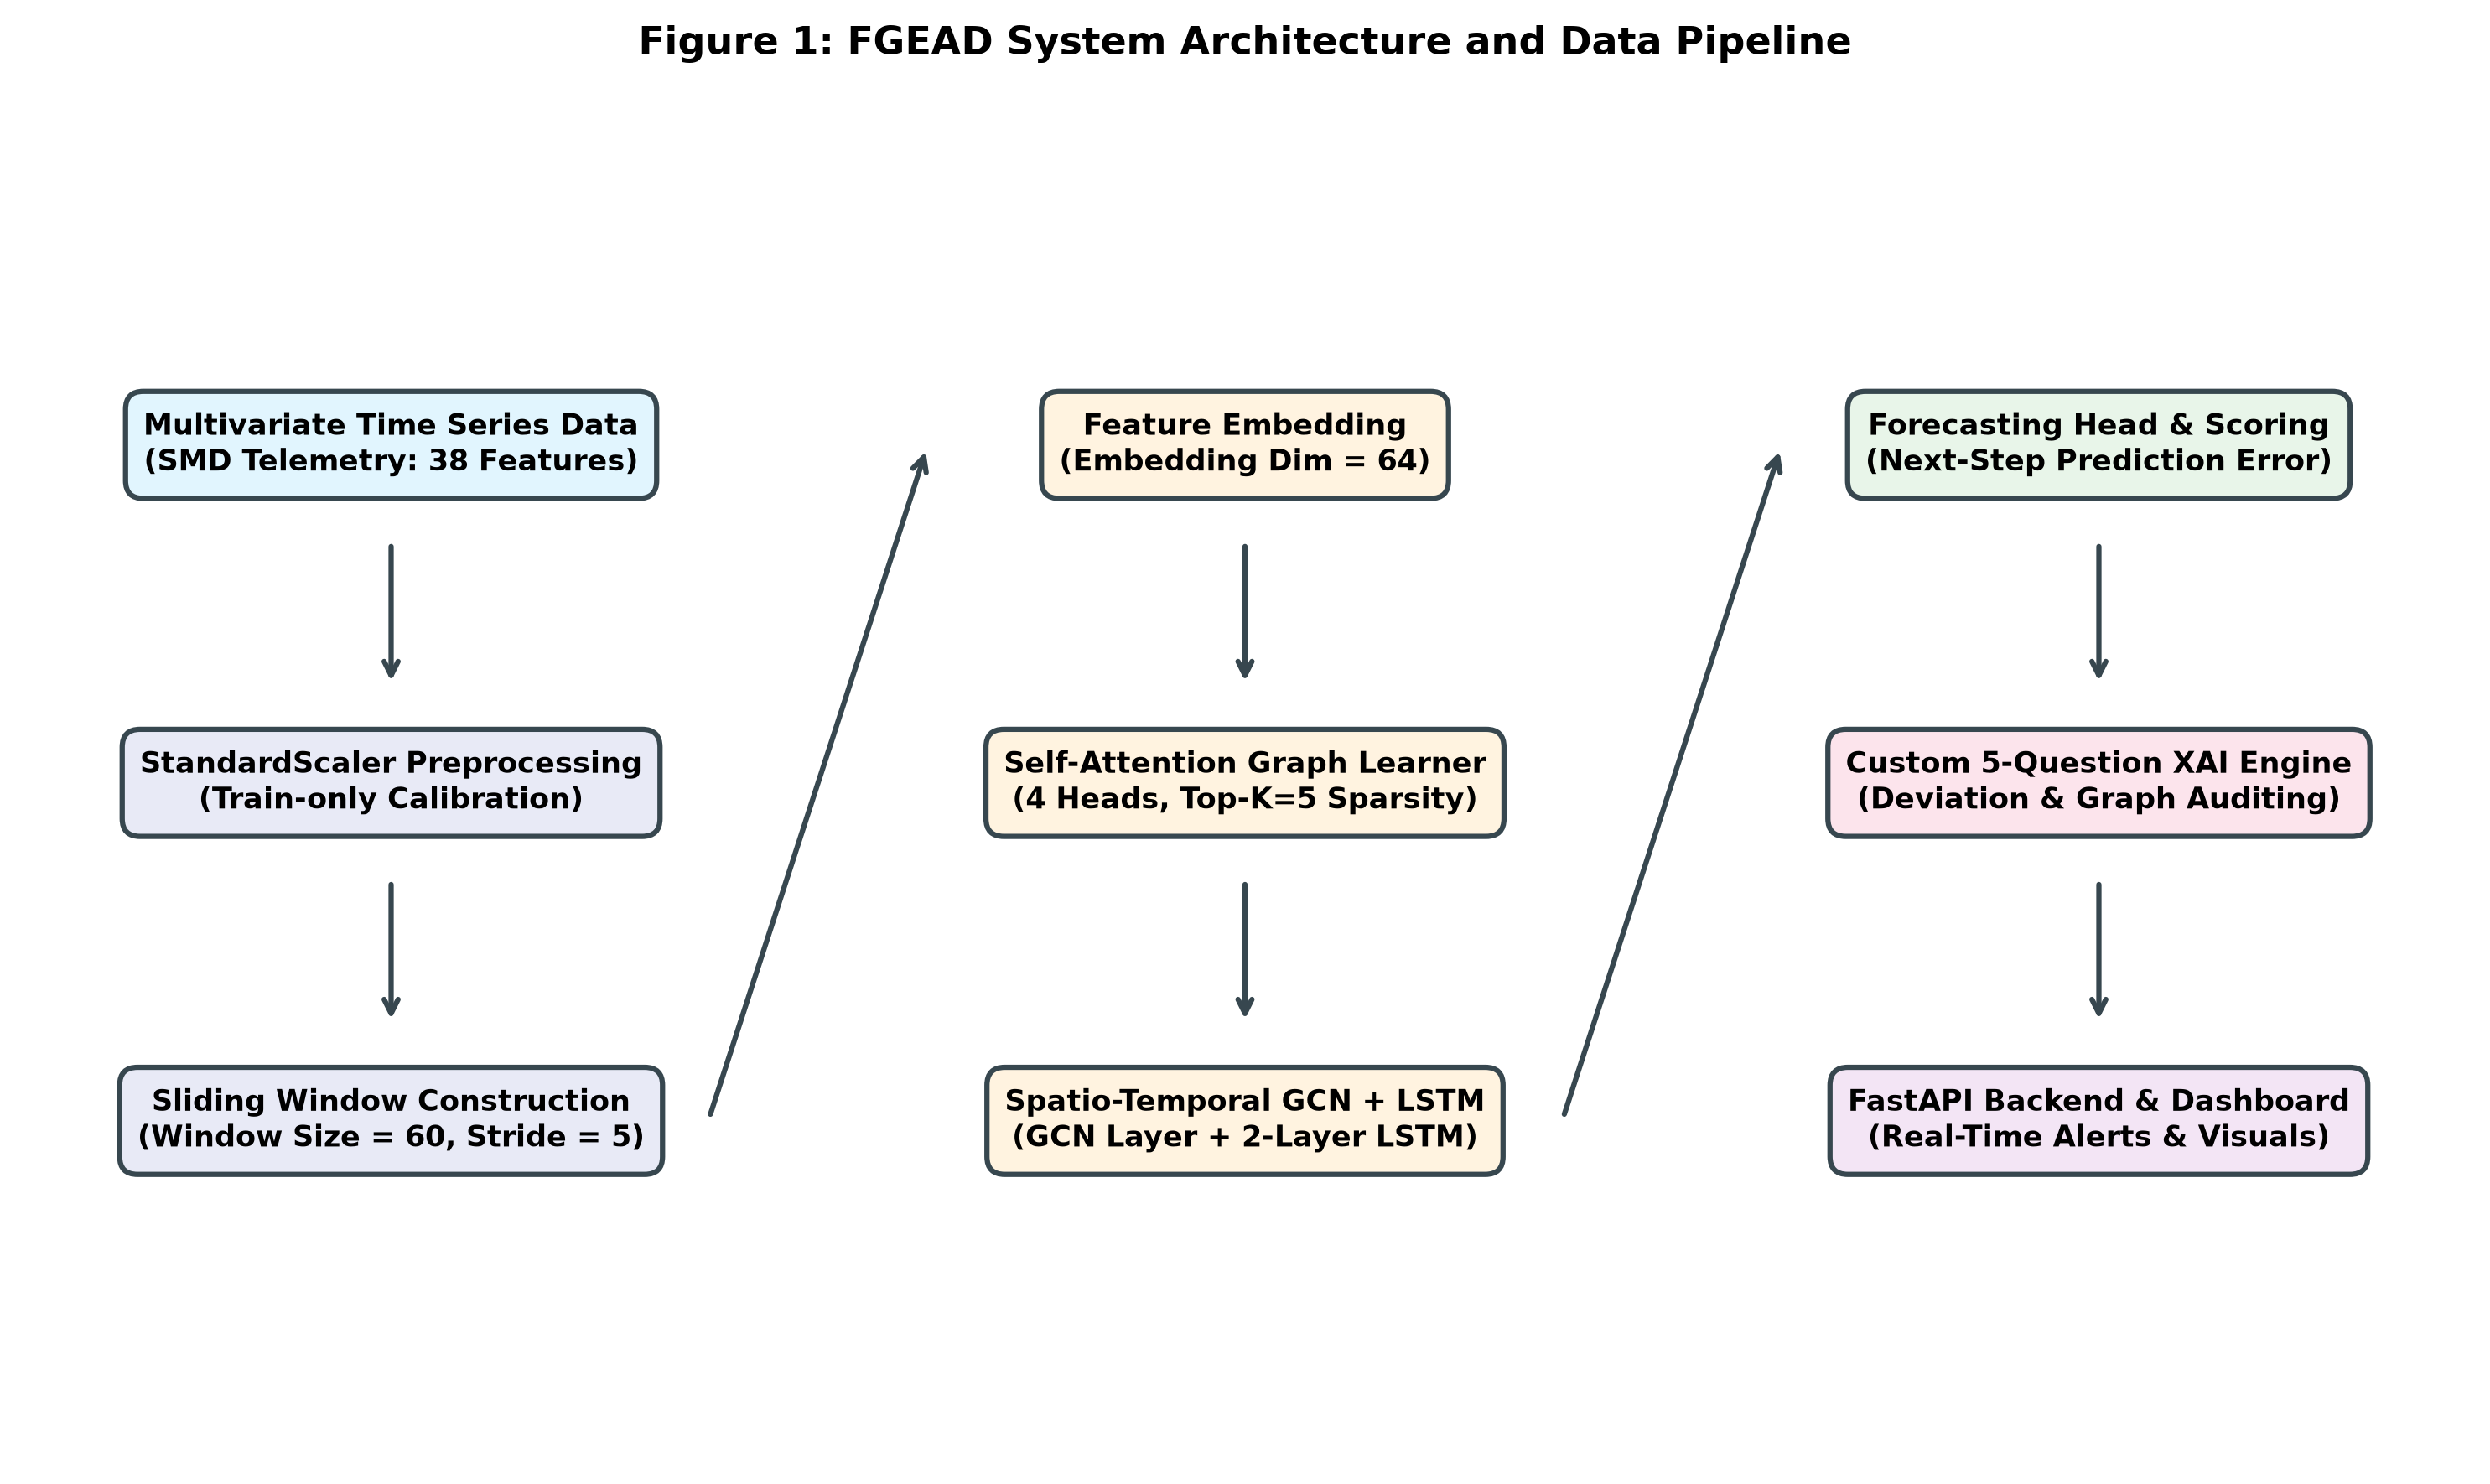
\includegraphics[width=0.92\textwidth]{figures/system_architecture.png}
\caption{Overall system architecture of FGEAD, depicting data ingestion, feature embedding, dynamic graph learning, spatio-temporal GCN+LSTM processing, next-step forecasting, anomaly scoring, and the 5-Question XAI Engine.}
\label{fig:architecture}
\end{figure*}

\subsection{Module 1: Feature Embedding}
Each metric index $i \in \{1, \dots, M\}$ is mapped to a dense trainable vector embedding $\mathbf{e}_i \in \mathbb{R}^{d}$ with dimension $d = 64$ using an embedding matrix $\mathbf{E} \in \mathbb{R}^{M \times d}$. The raw numerical metric values at timestep $t$ are projected into the embedding space, normalized via Layer Normalization, and passed through Dropout ($p=0.1$):
\begin{equation}
    \mathbf{H}^{(0)}_{t, i} = \text{LayerNorm}(\mathbf{e}_i \cdot x_{t, i}) \in \mathbb{R}^d
\end{equation}

\subsection{Module 2: Self-Attention Graph Learner}
To capture inter-metric dependencies without requiring a static predefined topology, FGEAD dynamically constructs a feature adjacency matrix $\mathbf{A} \in \mathbb{R}^{M \times M}$ using multi-head self-attention.

Temporal pooling is applied over the window length $T$: $\bar{\mathbf{h}}_i = \frac{1}{T}\sum_{t=1}^T \mathbf{H}^{(0)}_{t, i}$. Linear query ($\mathbf{W}_Q$) and key ($\mathbf{W}_K$) projections compute attention affinity scores across $H=4$ attention heads:
\begin{equation}
    \alpha_{ij}^{(h)} = \text{Softmax}\left( \frac{(\mathbf{W}_Q^{(h)} \bar{\mathbf{h}}_i) (\mathbf{W}_K^{(h)} \bar{\mathbf{h}}_j)^T}{\sqrt{d/H}} \right)
\end{equation}
The attention scores are averaged across heads to form a dense adjacency matrix $\tilde{\mathbf{A}} \in \mathbb{R}^{M \times M}$. To enforce graph sparsity and reduce noisy connections, a Top-$K$ hard mask ($K=5$) is applied per metric node, keeping only the top 5 strongest connections for each feature while zeroing out all others:
\begin{equation}
    \mathbf{A}_{ij} = \begin{cases} 
    \tilde{\mathbf{A}}_{ij}, & \text{if } \tilde{\mathbf{A}}_{ij} \in \text{Top-K}(\tilde{\mathbf{A}}_{i, :}) \\
    0, & \text{otherwise}
    \end{cases}
\end{equation}
An L1 sparsity regularization loss $\mathcal{L}_{\text{sparsity}} = \lambda \|\mathbf{A}\|_1$ ($\lambda = 10^{-4}$) is added during training.

\subsection{Module 3: Spatio-Temporal GCN + LSTM}
Spatial metric interactions are captured at each timestep $t$ via Graph Convolutional Networks (GCN):
\begin{equation}
    \mathbf{H}^{(1)}_t = \text{ReLU}\left( \text{BatchNorm1D}\left( \hat{\mathbf{A}} \mathbf{H}^{(0)}_t \mathbf{W}_{\text{GCN}} \right) \right)
\end{equation}
where $\hat{\mathbf{A}} = \mathbf{D}^{-1/2} (\mathbf{A} + \mathbf{I}_M) \mathbf{D}^{-1/2}$ is the symmetric normalized adjacency matrix and $\mathbf{W}_{\text{GCN}} \in \mathbb{R}^{d \times d}$ is learnable.

The spatial node representations at timestep $t$ are flattened into a vector of dimension $M \cdot d$ and fed sequentially into a 2-layer LSTM network with hidden state dimension $h_{\text{lstm}} = 128$ and dropout rate $0.2$:
\begin{equation}
    \mathbf{h}_t, (\mathbf{c}_t, \mathbf{s}_t) = \text{LSTM}\left( [\mathbf{H}^{(1)}_t], \mathbf{h}_{t-1} \right)
\end{equation}

\subsection{Module 4: Forecasting Head \& Anomaly Scoring}
The final LSTM hidden state $\mathbf{h}_T$ is mapped through a 2-layer MLP to predict the telemetry metrics at next timestep $T+1$:
\begin{equation}
    \hat{\mathbf{x}}_{T+1} = \mathbf{W}_2 \cdot \text{Dropout}\left( \text{ReLU}(\mathbf{W}_1 \mathbf{h}_T + \mathbf{b}_1) \right) + \mathbf{b}_2
\end{equation}
The absolute forecast error vector is $\mathbf{e}_{T+1} = |\mathbf{x}_{T+1} - \hat{\mathbf{x}}_{T+1}| \in \mathbb{R}^M$. FGEAD learns a trainable metric weighting parameter $\mathbf{w} \in \mathbb{R}^M$ normalized via Softmax: $\boldsymbol{\gamma} = \text{Softmax}(\mathbf{w})$. The overall scalar anomaly score for window $\mathbf{W}$ is:
\begin{equation}
    S_{\mathbf{W}} = \sum_{i=1}^M \gamma_i \cdot e_{T+1, i}
\end{equation}

The model is trained to minimize the combined forecasting and graph sparsity loss:
\begin{equation}
    \mathcal{L}_{\text{total}} = \frac{1}{B}\sum_{b=1}^B \|\mathbf{x}_b - \hat{\mathbf{x}}_b\|_2^2 + \lambda \|\mathbf{A}\|_1
\end{equation}

\section{Dataset and Preprocessing}

\subsection{Server Machine Dataset (SMD)}
The primary benchmark evaluated is the Server Machine Dataset (SMD) \cite{su2019omnianomaly}, collected from a large Internet enterprise over 5 weeks. SMD consists of 28 server machines across 3 clusters. We evaluate machine-1-1, which comprises 38 continuous telemetry metrics. The dataset details are summarized in Table~\ref{tab:dataset_summary}.

\begin{table}[h]
\caption{Dataset Characteristics of SMD Machine 1-1}
\label{tab:dataset_summary}
\centering
\begin{tabular}{ll}
\toprule
\textbf{Characteristic} & \textbf{Value / Setting} \\
\midrule
Machine ID & machine-1-1 \\
Total Features ($M$) & 38 metrics \\
Train Timesteps & 28,479 (100\% normal) \\
Test Timesteps & 28,479 \\
Test Anomaly Timesteps & 2,694 (Point anomaly rate: 9.46\%) \\
Window Size ($T$) & 60 timesteps \\
Window Stride & 5 timesteps \\
Train Windows & 5,684 windows \\
Test Windows & 5,684 windows \\
Test Anomaly Windows & 635 windows \\
\bottomrule
\end{tabular}
\end{table}

\subsection{Preprocessing Pipeline}
\begin{enumerate}
    \item \textbf{Missing Value Imputation:} Missing values are handled via forward-filling followed by backward-filling. Exact duplicate rows are removed.
    \item \textbf{Standardization:} Metrics are normalized using \texttt{StandardScaler}. To prevent data leakage, \texttt{fit()} is called exclusively on the training split ($\mathcal{D}_{\text{train}}$). Test sets are transformed using training mean $\boldsymbol{\mu}_{\text{train}}$ and standard deviation $\boldsymbol{\sigma}_{\text{train}}$.
    \item \textbf{Sliding Windowing:} Data is formatted into chronological sliding windows of size $T=60$ with stride $S=5$. Data is not shuffled to maintain temporal continuity.
    \item \textbf{Threshold Calibration:} A calibration subset (15\% of training windows) determines the anomaly threshold $\tau = 2.073376$ at the 99.5th percentile of normal prediction errors.
\end{enumerate}

\section{Machine Learning Model Setup}
FGEAD is implemented in PyTorch 2.0+. Training configurations and hyperparameter settings are detailed in Table~\ref{tab:model_config}.

\begin{table}[h]
\caption{FGEAD Hyperparameters and Training Configuration}
\label{tab:model_config}
\centering
\begin{tabular}{ll}
\toprule
\textbf{Hyperparameter} & \textbf{Value} \\
\midrule
Embedding Dimension ($d$) & 64 \\
Self-Attention Heads ($H$) & 4 \\
Top-$K$ Graph Connections & 5 per metric \\
Sparsity Regularization ($\lambda$) & $10^{-4}$ \\
GCN Output Dimension & 64 \\
LSTM Layers / Hidden Dim & 2 layers / 128 units \\
LSTM Dropout & 0.2 \\
MLP Hidden Layer & 64 units \\
Optimizer & Adam ($\text{lr}=10^{-3}$, weight decay $10^{-4}$) \\
Learning Rate Scheduler & ReduceLROnPlateau (factor 0.5, patience 3) \\
Batch Size / Epochs & 64 / 30 epochs \\
Gradient Clipping & Max norm = 1.0 \\
Early Stopping & Patience = 7 epochs \\
\bottomrule
\end{tabular}
\end{table}

\section{Explainable AI Framework}

When an anomaly is flagged ($S_{\mathbf{W}} > \tau$), FGEAD triggers its custom 5-Question Explainability Engine (\texttt{models/explainer.py}). Crucially, model inputs and predictions are inverse-transformed back to the original scale prior to evaluation, ensuring scale-consistent explanations.

\subsection{Q1: Metric Deviation Ranking}
At peak anomaly timestep $t^* = \arg\max_{t} S_t$, the absolute error for feature $i$ is calculated as $d_i = |x_{t^*, i} - \hat{x}_{t^*, i}|$. Deviations are standardized into Z-scores using historical window standard deviation: $z_i = d_i / \sigma_{W, i}$. Features are ranked by $z_i$, and the top $K=5$ metrics are isolated.

\subsection{Q2: Directional Deviation Labeling}
Comparing actual value $x_{t^*, i}$ against predicted $\hat{x}_{t^*, i}$ on the original metric scale yields a semantic directional label:
\begin{equation}
    \text{Label}_i = \begin{cases}
    \text{``}\uparrow \text{ spike''}, & \text{if } x_{t^*, i} - \hat{x}_{t^*, i} > +0.1 \sigma_i \\
    \text{``}\downarrow \text{ drop''}, & \text{if } x_{t^*, i} - \hat{x}_{t^*, i} < -0.1 \sigma_i \\
    \text{``}\approx \text{ stable''}, & \text{otherwise}
    \end{cases}
\end{equation}

\subsection{Q3: Graph Relationship Auditing}
To audit inter-metric structural shifts, FGEAD isolates the window surrounding the peak anomaly ($t^* \pm 10$ steps) and computes its empirical Pearson correlation matrix $\mathbf{R}^{\text{obs}} \in \mathbb{R}^{M \times M}$. This is contrasted against the model's learned attention-derived dependency matrix $\mathbf{A} \in \mathbb{R}^{M \times M}$.

Graph Relationship Auditing measures discrepancies between the model's learned dependency representation and observed empirical co-movement. It does not perform causal discovery or claim causal proof. A relationship change is flagged for pair $(i, j)$ if $|\mathbf{R}^{\text{obs}}_{ij} - \mathbf{A}_{ij}| \ge 0.20$. Relationship break types are categorized into:
\begin{itemize}
    \item \textbf{Complete Decoupling:} $\mathbf{A}_{ij} \ge 0.70$ (strong expected dependency) but $\mathbf{R}^{\text{obs}}_{ij} < 0.10$.
    \item \textbf{Sign Reversal:} $\mathbf{A}_{ij} \ge 0.20$ but $\mathbf{R}^{\text{obs}}_{ij} < 0$.
    \item \textbf{Relationship Change:} Generic gap $|\mathbf{R}^{\text{obs}}_{ij} - \mathbf{A}_{ij}| \ge 0.20$.
\end{itemize}
Severity ratings are assigned: CRITICAL (gap $\ge 0.70$), HIGH (gap $\ge 0.50$), MEDIUM (gap $\ge 0.20$).

\subsection{Q4: Temporal Range Localization}
Contiguous anomalous timesteps within the window are identified to bound the anomaly start time $t_{\text{start}}$, end time $t_{\text{end}}$, and duration in timesteps and minutes.

\subsection{Q5: Composite Alert Confidence Calibration}
A composite confidence score $C \in [0, 1.0]$ is computed using a weighted combination of four normalized signal components:
\begin{equation}
    C = w_s \cdot S_{\text{signal}} + w_d \cdot D_{\text{signal}} + w_f \cdot F_{\text{signal}} + w_g \cdot G_{\text{signal}}
\end{equation}
where $w_s = 0.40, w_d = 0.25, w_f = 0.20, w_g = 0.15$. The four normalized signal components are calculated in the implementation as:
\begin{align}
    S_{\text{signal}} &= \min\left(1.0, \max\left(0.0, \frac{S_{\text{peak}} - \tau}{0.25 \tau}\right)\right) \\
    D_{\text{signal}} &= \min\left(1.0, \frac{\text{Duration}}{0.30 \cdot T}\right) \\
    F_{\text{signal}} &= \min\left(1.0, \frac{N_{\text{deviating}}}{0.30 \cdot M}\right) \\
    G_{\text{signal}} &= \min\left(1.0, \frac{N_{\text{broken}}}{0.20 \cdot E_{\text{total}}}\right)
\end{align}
Confidence scores translate into discrete operational alert levels: CRITICAL ($\ge 80\%$), HIGH ($\ge 60\%$), MEDIUM ($\ge 40\%$), and LOW ($< 40\%$).

\section{System Architecture and Implementation}

FGEAD is designed as a deployment-oriented microservice prototype. The backend is implemented using FastAPI (\texttt{api/main.py}) and Uvicorn, providing RESTful endpoints:
\begin{itemize}
    \item \texttt{GET /health}: System status, active execution device (CPU/CUDA), loaded model configuration, and feature counts.
    \item \texttt{GET /dataset}: Dataset statistics, train/test sample counts, and baseline anomaly rates.
    \item \texttt{GET /machine}: Active machine metadata and metric feature names.
    \item \texttt{POST /predict}: Accepts a $60 \times 38$ telemetry window tensor input and returns a JSON payload containing prediction status, anomaly scores, top 5 feature Z-scores, broken graph pairs, alert confidence level, and synthesized diagnostic root-cause hypothesis string. Execution latency is handled via lightweight HTTP REST calls.
\end{itemize}

The frontend is built using Streamlit (\texttt{app/streamlit\_app.py}), delivering an observability dashboard prototype. It visualizes interactive Plotly telemetry timelines, ground-truth anomaly bands, actual vs. forecast profile charts, HTML tables with Z-score progress bars, and graph relationship break tables.

\section{Experimental Results and Evaluation}

\subsection{Evaluation Metrics}
Model performance is evaluated using standard metrics: Precision ($P$), Recall ($R$), F1-Score ($F_1$), Area Under the ROC Curve (ROC-AUC), and Area Under the Precision-Recall Curve (PR-AUC). Evaluations are conducted at both \textbf{Window Level} and \textbf{Point Level} (applying a minimum anomaly duration smoothing filter of 5 steps).

\subsection{Quantitative Results on SMD Machine 1-1}
Table~\ref{tab:smd_results} presents the official evaluation results on SMD Machine 1-1 across 28,479 test timesteps (5,684 test windows).

\begin{table}[h]
\caption{FGEAD Experimental Performance Results on SMD Machine 1-1}
\label{tab:smd_results}
\centering
\begin{tabular}{lcc}
\toprule
\textbf{Evaluation Metric} & \textbf{Window-Level} & \textbf{Point-Level} \\
\midrule
Threshold ($\tau$) & 2.073376 & 2.073376 \\
Precision ($P$) & 0.5600 & 0.4891 \\
\textbf{Recall ($R$)} & \textbf{0.9039} & \textbf{0.9714} \\
F1-Score ($F_1$) & 0.6916 & 0.6506 \\
\textbf{ROC-AUC} & \textbf{0.9709} & \textbf{0.9708} \\
PR-AUC & 0.7981 & 0.7373 \\
True Anomaly Timesteps & — & 2,694 \\
Detected Anomaly Timesteps & — & 5,351 \\
\bottomrule
\end{tabular}
\end{table}

On a secondary 20-feature synthetic telemetry dataset (5,000 steps), FGEAD achieved Precision = 0.7273, Recall = 0.8571, F1 = 0.7869, and ROC-AUC = 0.9501.

\subsection{Discussion of Precision-Recall Trade-off}
As shown in Table~\ref{tab:smd_results}, FGEAD exhibits strong discriminative performance (ROC-AUC 0.9709) and high recall (0.9039 window-level, 0.9714 point-level). The moderate precision (0.5600) and F1-score (0.6916) stem directly from the 99.5th percentile train-only threshold calibration strategy. In an operational monitoring setting where missed anomalies may be costly, a high-recall threshold can be a reasonable design choice prioritizing anomaly sensitivity over precision.

\section{XAI Case Study and Diagnostic Hypothesis Analysis}

To illustrate FGEAD's explainability in action, we extract an actual anomalous test window from SMD Machine 1-1 centered around peak timestep $t^* = 17489$ (window score $S = 1949.62$, threshold $\tau = 2.073$).

\begin{table}[h]
\caption{FGEAD Diagnostic Case Study Output (Peak $t^* = 17489$)}
\label{tab:case_study}
\centering
\begin{tabular}{lccccc}
\toprule
\textbf{Feature Name} & \textbf{Actual} & \textbf{Predicted} & \textbf{Deviation} & \textbf{Z-Score} & \textbf{Label} \\
\midrule
\texttt{feature\_33} & 1.0000 & 0.0000 & 1.0000 & $3.7\sigma$ & $\uparrow$ spike \\
\texttt{feature\_28} & 1.0000 & 0.0001 & 0.9999 & $3.8\sigma$ & $\uparrow$ spike \\
\texttt{feature\_32} & 1.0000 & 0.0003 & 0.9997 & $3.7\sigma$ & $\uparrow$ spike \\
\texttt{feature\_24} & 1.0000 & 0.0600 & 0.9400 & $3.6\sigma$ & $\uparrow$ spike \\
\texttt{feature\_31} & 1.0000 & 0.0886 & 0.9114 & $3.7\sigma$ & $\uparrow$ spike \\
\bottomrule
\end{tabular}
\end{table}

\textbf{Graph Auditing Findings:} The Graph Relationship Auditor identified 49 changed feature pairs. Top broken pairs included:
\begin{itemize}
    \item \texttt{feature\_13} $\leftrightarrow$ \texttt{feature\_27}: Expected dependency $= 0.14$, Observed correlation $= 0.92$ (\texttt{RELATIONSHIP CHANGE}).
    \item \texttt{feature\_10} $\leftrightarrow$ \texttt{feature\_15}: Expected dependency $= 0.25$, Observed correlation $= 1.00$ (\texttt{RELATIONSHIP CHANGE}).
\end{itemize}

\textbf{Alert \& Diagnostic Hypothesis Synthesis:} The engine computed an Alert Confidence of \textbf{72.1\%} (\textbf{HIGH ALERT LEVEL}) and generated the diagnostic hypothesis:
\textit{``Unusual multivariate pattern detected: feature\_33 $\uparrow$ spike, feature\_28 $\uparrow$ spike, feature\_32 $\uparrow$ spike, feature\_13/feature\_27 relationship change.''} Because SMD does not provide metric-level root-cause annotations, this output represents a candidate diagnostic hypothesis rather than confirmed physical causation.

\section{Qualitative Literature Synthesis}

Table~\ref{tab:comparison} provides a qualitative synthesis comparing the methodological characteristics of FGEAD against major published architectures reviewed in the literature. This table summarizes design traits reported in published works and is not a controlled benchmark under identical experimental setups.

\begin{table*}[t]
\caption{Qualitative Literature Synthesis of Methodological Characteristics}
\label{tab:comparison}
\centering
\begin{tabular}{lcccccc}
\toprule
\textbf{Study / Method} & \textbf{ML Architecture} & \textbf{Target Domain} & \textbf{XAI Mechanism} & \textbf{Feature Explanation} & \textbf{Graph Auditing} & \textbf{Deployment} \\
\midrule
OmniAnomaly \cite{su2019omnianomaly} & Stochastic RNN + NormFlow & SMD, SMAP & Rec. Prob. & Score Ranking & No & Script \\
USAD \cite{audibert2020usad} & Adversarial Autoencoder & SMD, SWaT & None & None & No & Script \\
MSCRED \cite{zhang2019deep} & ConvLSTM + SigMatrix & Synthetic, Power & SigMatrix & Image Residuals & Dense Correlation & Script \\
GDN \cite{deng2021graph} & GNN + Structure Learning & SWaT, WADI & Learned Graph & Attention Weights & Implicit Deviation & Script \\
MTAD-GAT \cite{zhao2020multivariate} & Graph Attention Network & SMD, MSL & Dual Attention & Attention Weights & No & Script \\
InterFusion \cite{li2021multivariate} & Hierarchical VAE & SMD, SMAP & MCMC Sampling & Metric Localization & No & Script \\
Anomaly Trans. \cite{xu2022anomaly} & Transformer + Association & SMD, SWaT & Assoc. Disc. & Temporal Attention & No & Script \\
\textbf{FGEAD (Ours)} & \textbf{Self-Attn GCN + LSTM} & \textbf{SMD Telemetry} & \textbf{5-Q Engine} & \textbf{Z-Score + Dir ($\uparrow/\downarrow$)} & \textbf{Explicit Graph Audit} & \textbf{FastAPI + Streamlit} \\
\bottomrule
\end{tabular}
\end{table*}

\section{Limitations}
A comprehensive assessment identifies several genuine limitations:
\begin{enumerate}
    \item \textbf{Single-Machine Evaluation Scope:} Only SMD Machine 1-1 is evaluated in detail; multi-machine generalization across all 28 SMD servers remains to be established.
    \item \textbf{Lack of Annotated Ground-Truth Root Causes:} SMD provides ground-truth temporal anomaly labels but lacks feature-level root-cause annotations, preventing quantitative evaluation of explanation accuracy.
    \item \textbf{Generic Metric Semantics:} SMD metrics are named generically (\texttt{feature\_00} to \texttt{feature\_37}), limiting semantic natural-language diagnosis to keyword heuristics.
    \item \textbf{Non-Causal Auditing Nature:} Graph Relationship Auditing measures discrepancy between dependency representations and empirical correlations; it should not be interpreted as proving physical causality.
    \item \textbf{Heuristic Confidence Scoring:} The alert confidence score is an operational heuristic and has not been externally calibrated against probabilistic ground-truth outcomes.
    \item \textbf{Quadratic Correlation Complexity:} Computing $M \times M$ Pearson correlation matrices for anomalous windows incurs $\mathcal{O}(M^2 T)$ complexity, which can create bottlenecks for large metric counts ($M > 500$).
    \item \textbf{Synthetic Dataset Scope:} The 20-feature synthetic dataset provides controlled validation but does not substitute for diverse real-world industrial benchmarks.
\end{enumerate}

\section{Future Work}
Future research directions include: (1) evaluating FGEAD across all 28 SMD server machines and external industrial datasets, (2) benchmarking explanation quality on datasets with labeled root causes such as Exathlon \cite{jacob2021exathlon}, (3) calibrating confidence scores against operator feedback, (4) incorporating adaptive/seasonal thresholding, (5) optimizing graph auditing via sparse correlation computations, and (6) integrating semantic metric metadata for operational deployments.

\section{Conclusion}
We presented \textbf{FGEAD}, a feature-level graph-based explainable anomaly detection framework for multivariate server telemetry. By combining self-attention graph learning, GCN, and LSTM with a structured 5-Question XAI engine, FGEAD bridges the gap between high-sensitivity anomaly forecasting and actionable operational diagnostics. Evaluated on SMD Machine 1-1, FGEAD achieved a window-level ROC-AUC of 0.9709 and Point-level Recall of 0.9714. The system provides operations teams with transparent Z-score rankings, directional indicators, graph relationship auditing, and calibrated alert confidence levels delivered through a FastAPI REST backend and Streamlit dashboard prototype.

\bibliographystyle{IEEEtran}
\bibliography{references}

\end{document}

